\documentclass[10pt]{beamer}
\usetheme[background=light,block=fill,progressbar=foot]{metropolis}
%\usepackage[UTF8]{ctex}
\usepackage{graphicx}
\usepackage{caption}
\usepackage{bm}
\usepackage{booktabs}
\usepackage{natbib}
\newcommand{\supercite}[1]{\textsuperscript{\textsuperscript{\cite{#1}}}}
\newcommand{\emoji}[1]{\text{\raisebox{-0.2em}{\includegraphics[height=1em]{emojis/#1.png}}}}
%\usefonttheme[onlymath]{serif}

\begin{document}
	\title{Deep Learning Book}
	\subtitle{Chapter 6 \\ Deep Feedforward Networks}
	\author{Botian Shi \\ botianshi@bit.edu.cn}
	\date{\today}

	\begin{frame}[plain]
		\titlepage
	\end{frame}

	\begin{frame}
		You can download the \LaTeX\, source code of this file from \href{https://github.com/friskit-china/DLBookSlides}{\underline{Here}}.
	\end{frame}
	
	\begin{frame}{Feedforward Networks}
		
		\begin{itemize}
			\item A type of neural network
				\begin{itemize}
					\item \emph{Deep feedforward network}
					\item \emph{feedforward neural network}
					\item \emph{multilayer perceptron (MLP)}
				\end{itemize}
			\item For a classifier, $y = f^{\,*}(\bm{x})$ maps an input $\bm{x}$ to category $\bm{y}$
			\item Defines a mapping:
					\begin{center}
						$\bm{y}=f(\bm{x};\bm{\theta})$
					\end{center}
			\item Learns the best approximation of $f^{\,*}$ with parameter $\bm{\theta}$
			\item Feedforward only, no feedback connections.
			\item The basis of many applications.
		\end{itemize}
	\end{frame}

	\begin{frame}{Feedforward networks are ...}
		\begin{enumerate}
			\item Extreme important.
			\item Stepping stone on the path to recurrent neural networks.
		\end{enumerate}
		\begin{exampleblock}{Example: convolutional neural network}
			\begin{figure}
				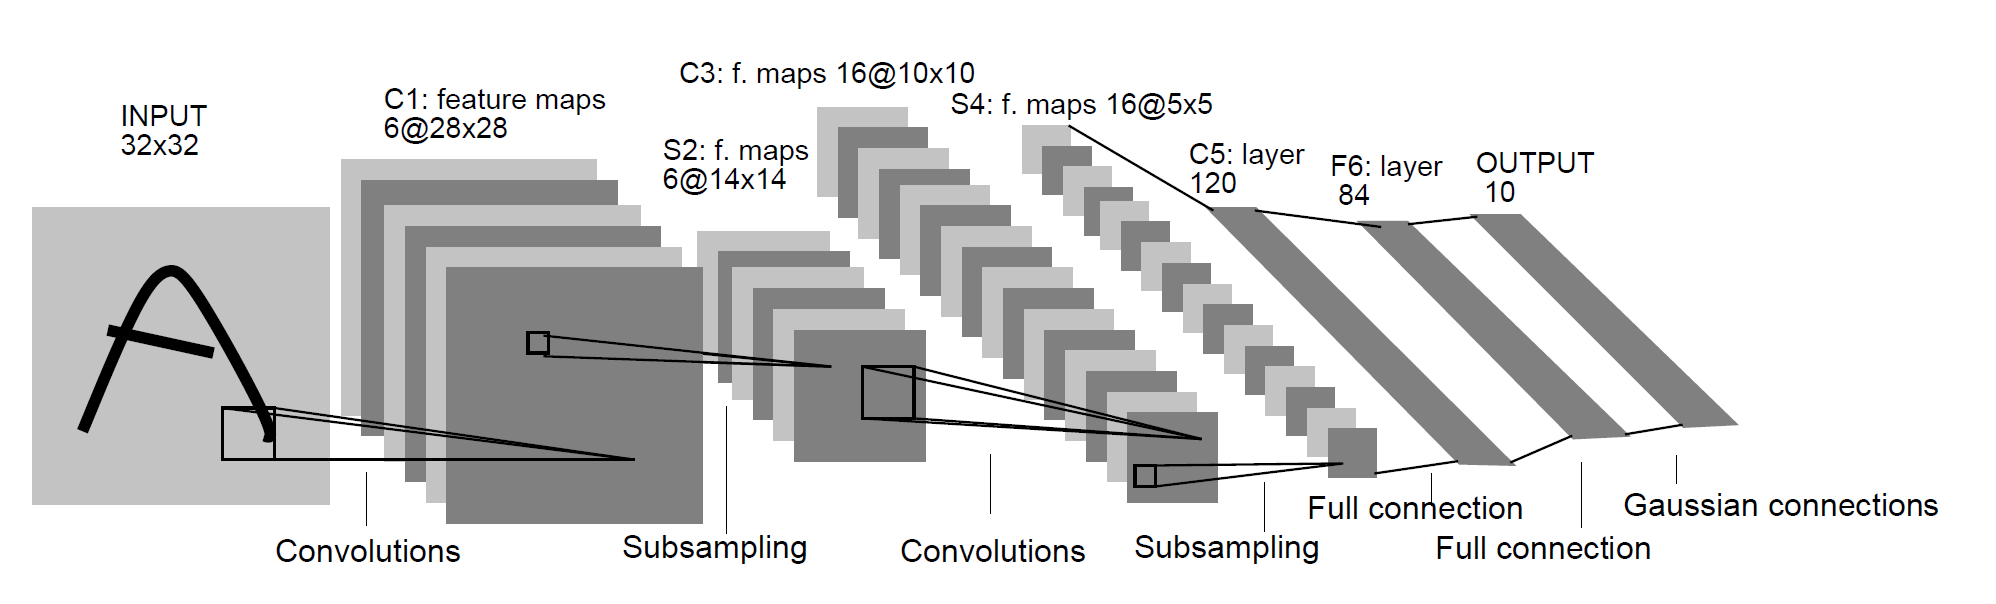
\includegraphics[width=25em]{figures/lenet-5.png}
				\caption{A type of convolutional neural network: \\ LeNet-5 (\citet{lecun1998gradient})}
			\end{figure}
		\end{exampleblock}
	\end{frame}

	\begin{frame}{Multilayer Perceptron}
		\begin{columns}[T,onlytextwidth]
			\column{0.7\textwidth}
			\begin{itemize}
				\item Why called \emph{networks}?
				\begin{itemize}
					\item Composing together many different functions.
					\item Model is associated with a DAG describing the composition.
					\begin{equation*}
					f(\bm{x}) = f^{\,(3)\,}(f^{\,(2)\,}(f^{\,(1)\,}(\bm{x})))
					\end{equation*}
					\item $f^{\,(1)\,}$ called first layer of the network
					\item $f^{\,(2)\,}$ called second layer, and so on
					\item $f^{\,(2)\,}$ called output layer
				\end{itemize}
			\end{itemize}
			\column{0.3\textwidth}
			\begin{figure}
				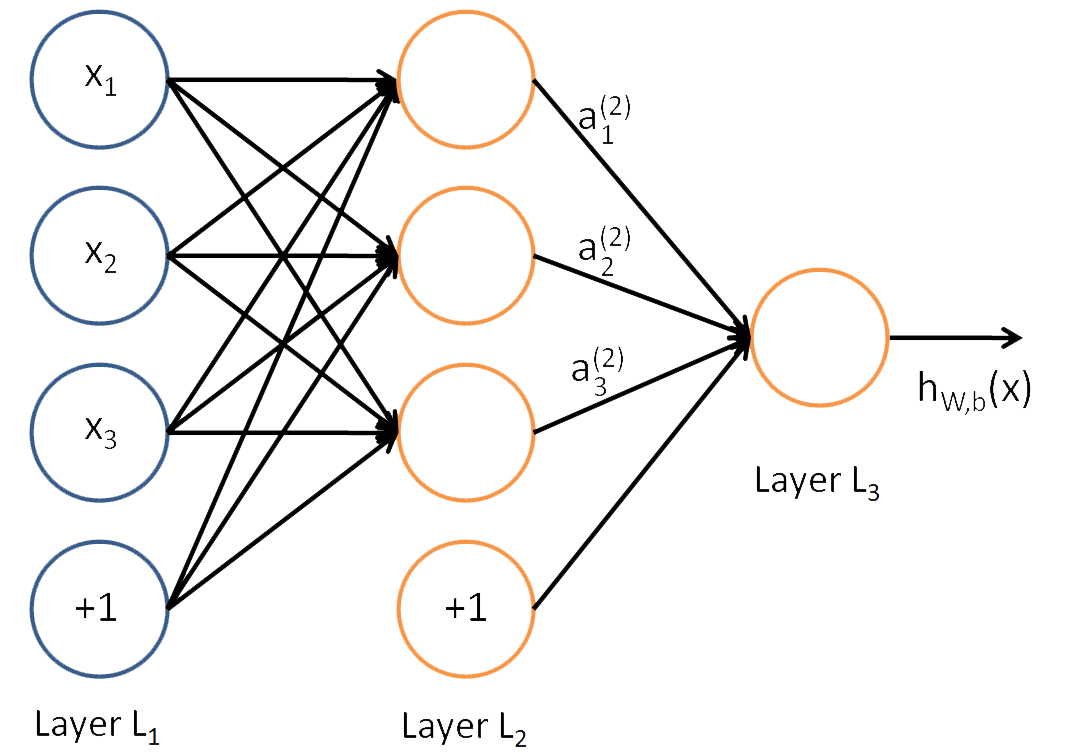
\includegraphics[width=10em]{figures/multilayer-perceptron.png}
				\caption{\\ An example of MLP  (from \href{http://ufldl.stanford.edu/wiki/index.php/File:Network331.png}{UFLDL})}
			\end{figure}
		\end{columns}
		\begin{itemize}
			\item During training, we drive $f\,(\bm{x})$ to match $f^{\,*}(\bm{x})$
			\item Each example $\bm{x}$ is accompanied by a label $y\approx f^{\,*}(\bm{x})$
			\item At each point $\bm{x}$, network must produce a value that is close to $\bm{y}$.
			\item The learning algorithm must decide how to use those layers to produce the desired output.
			\item Layers between input and output layer are called \emph{hidden layer}.
		\end{itemize}
	\end{frame}

	\begin{frame}{The \emph{NEURAL} network}
		\begin{itemize}
			\item Inspired by neuroscience.
			\begin{columns}
				\column{0.5\textwidth}
				\begin{figure}
					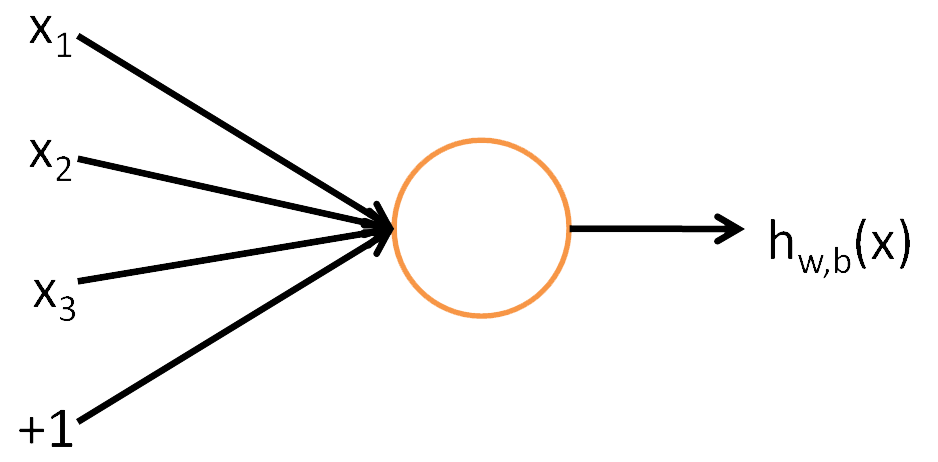
\includegraphics[height=5em]{figures/neuron.png}
					\caption{Neuron (from \href{http://deeplearning.stanford.edu/wiki/index.php/File:SingleNeuron.png}{UFLDL})}
				\end{figure}
			
				\column{0.5\textwidth}
				\begin{figure}
					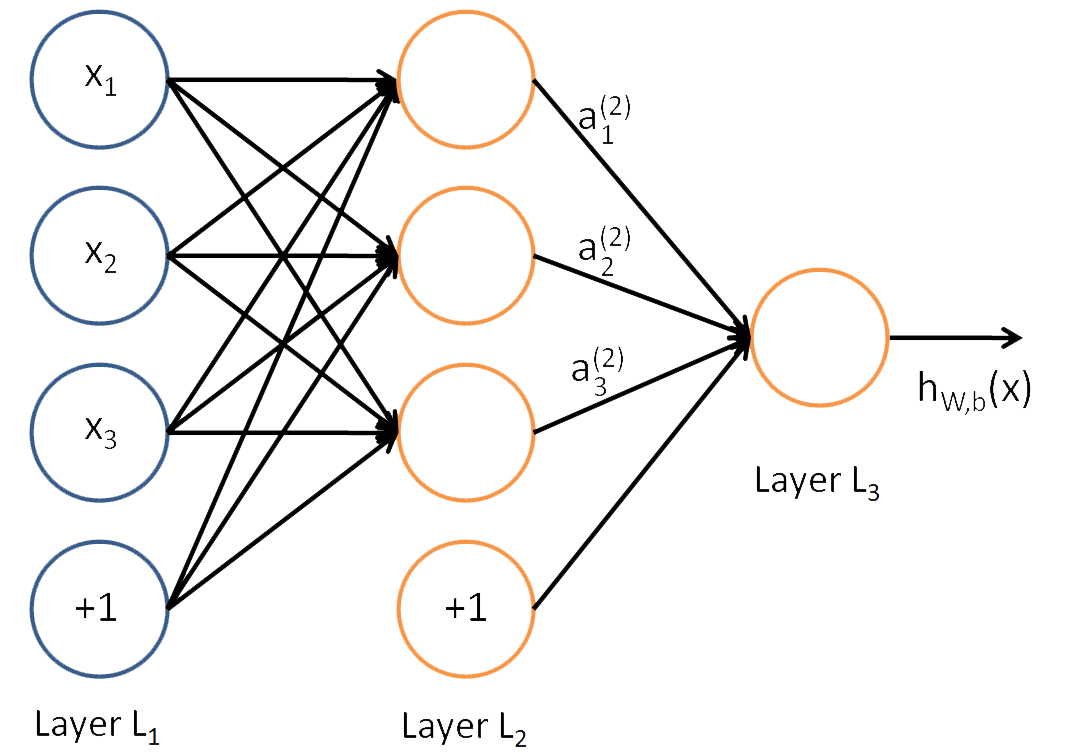
\includegraphics[height=5em]{figures/multilayer-perceptron.png}
					\caption{MLP (from \href{http://ufldl.stanford.edu/wiki/index.php/File:Network331.png}{UFLDL})}
				\end{figure}
					
			\end{columns}
			\item Each hidden layer is vector-valued. The dimensionality of these hidden layers determines the \emph{width} of the model.
			\item Each element of the vector may be interpreted as a neuron.
			\item Layer consist of many \emph{units} that act in parallel, each representing a vector-to-scalar function.
			\item Each unit resembles a neuron that receives input from many other units and computes its own activation value.
		\end{itemize}
	\end{frame}

	\begin{frame}{The \emph{NEURAL} network}
		\begin{itemize}
			\item The idea of using many layers of vector-valued representation is drawn from neuroscience.
			\item Modern neural network research $\ne$ perfectly model the brain.
			\item Feedforward networks $\approx$ function approximation machines.
			\item Inspired by brain, rather than model a brain.
		\end{itemize}
	\end{frame}
	
	\begin{frame}{Understand feedforward networks}
		\begin{itemize}
			\item Linear Models
			\begin{exampleblock}{Linear Regression}
				\vspace{-2em}
				\begin{center}
					$$h_\theta(\bm{x};\theta)=\theta ^T\bm{x}=\theta_0+\theta_1x_1+\theta_2x_2+\dots+\theta_nx_n$$	
					\vspace{-2em}
					$$\theta=\mathop{\arg\min}_{\theta}\mathrm{J}(\theta;\bm{X})=\mathop{\arg\min}_{\theta}\frac{1}{2}\sum^{m}_{i=1}(h_\theta(x^{(i)})-y^{(i)})^2$$
					\vspace{-1em}
				\end{center}
			\end{exampleblock}
			
			\begin{exampleblock}{Logistic Regression}
				\vspace{-1.5em}
				\begin{center}
					$$h_\theta(\bm{x};\theta)=g(\theta^T\bm{x})=\frac{1}{1+e^{-\theta^T\bm{x}}}$$
					\vspace{-1.5em}
					$$g(z)=\frac{1}{1+e^{-z}}$$
					\vspace{-1.5em}
				\end{center}
			\end{exampleblock}
			
			\begin{exampleblock}{General Linear Model}
				$$p(y;\eta)=b(u)\exp(\eta^TT(y)-a(\eta))$$
			\end{exampleblock}
		\end{itemize}
		
	\end{frame}
	
	\begin{frame}{Understand feedforward networks}
		\begin{itemize}
			\item Efficiently and reliable
			\item The model capacity is limited to linear functions.
			\begin{itemize}
				\item The model cannot understand the interaction between any two input variables.
			\end{itemize}
			\item To extend linear models to represent nonlinear functions of $\bm{x}$, we can apply the linear model not to $\bm{x}$ itself but to a transformed input $\phi(\bm{x})$, where $\phi$ is a \emph{nonlinear transformation}.
			\item $\phi$ provide a set of features describing $\bm{x}$, or provide a new representation fo $\bm{x}$
		\end{itemize}
	\end{frame}
	
	\begin{frame}{Understand feedforward networks}
		\begin{itemize}
			\item How to choose $\phi$?
			\begin{enumerate}
				\item Use a very generic $\phi$, e.g., infinite-dimensional $\phi$.
				\begin{itemize}
					\item \emoji{1F642} High dimension $\Leftrightarrow$ enough capacity to fit the training set. 
					\item \emoji{1F641} High dimension $\Leftrightarrow$ poor generalization capacity.
					\item \emoji{1F641} More is less: Runge phenomenon; Gibbs phenomenon.
%					\begin{figure}
%						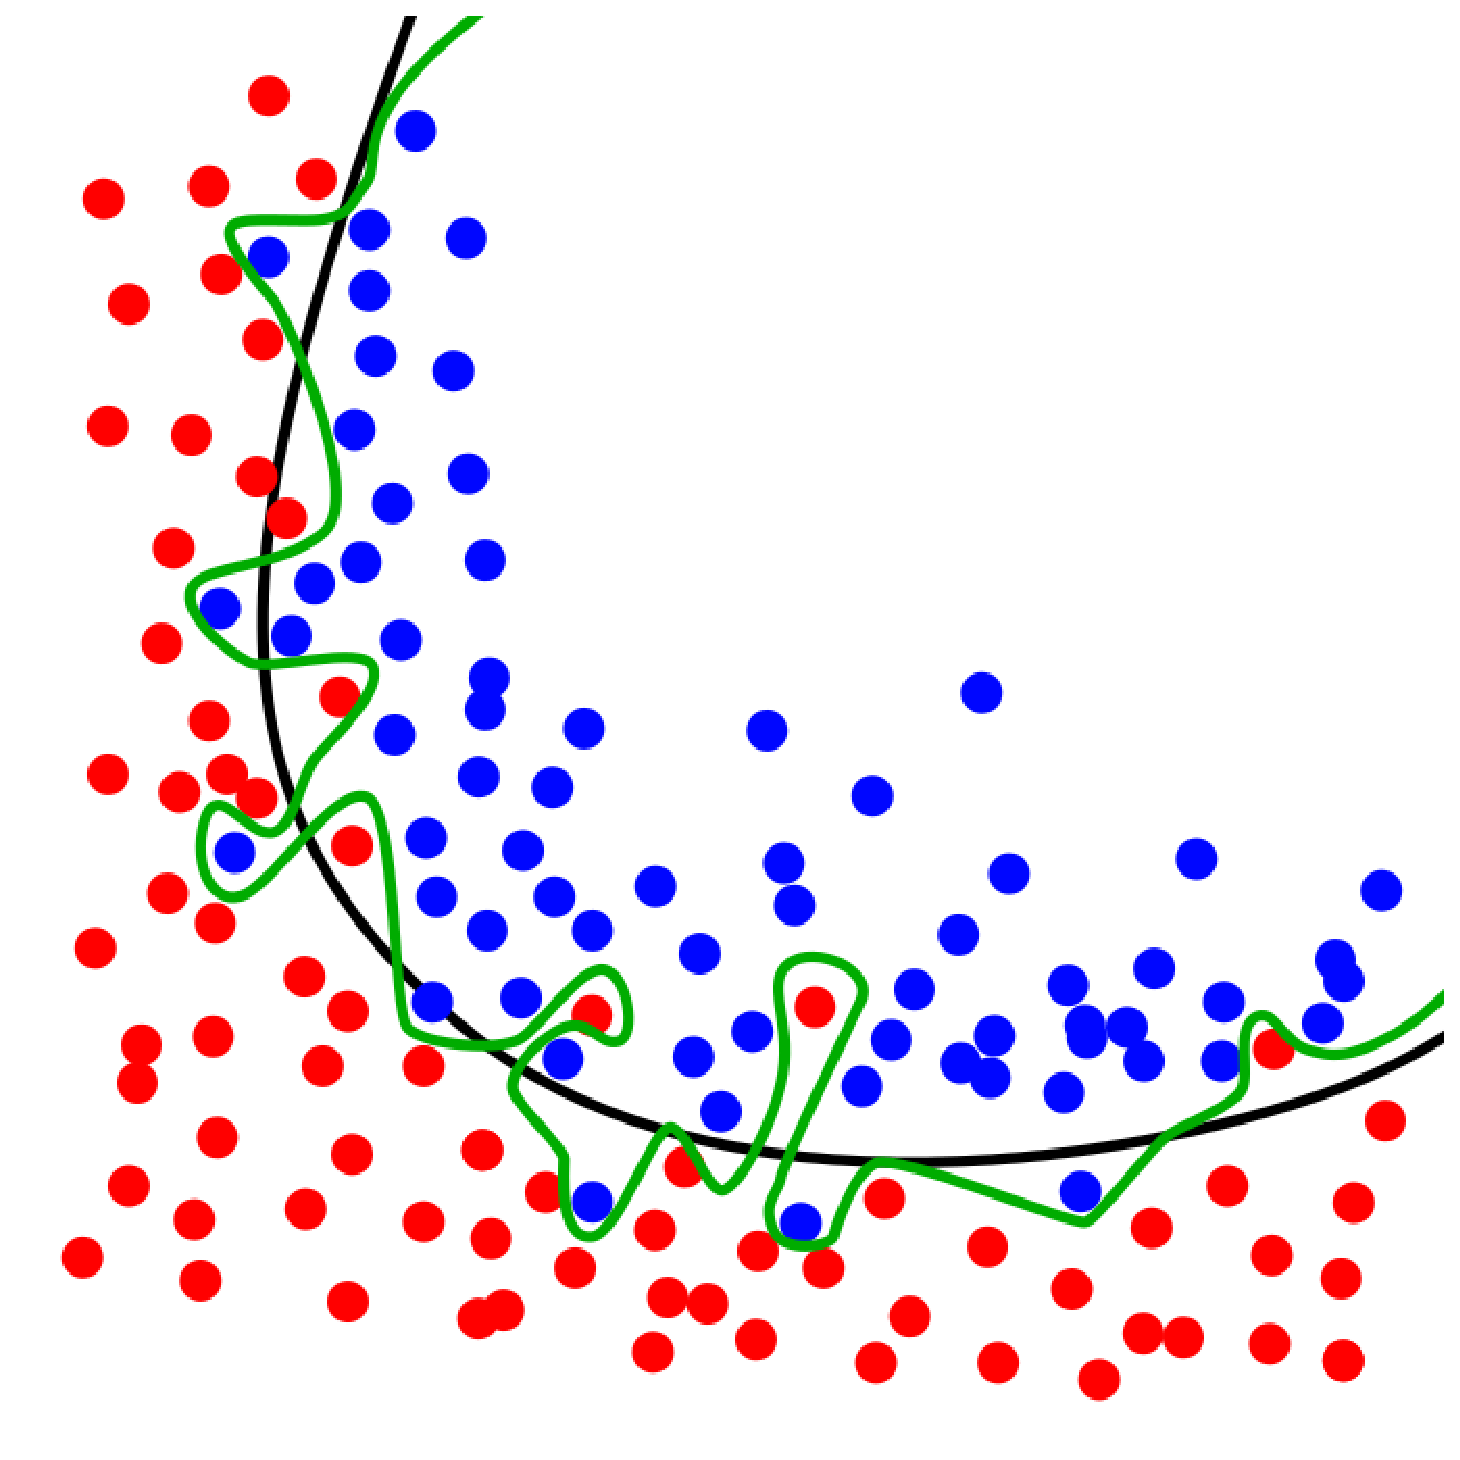
\includegraphics[height=10em]{figures/overfitting.eps}
%						\caption{Overfitting (from: \href{https://commons.wikimedia.org/wiki/File:Overfitting.svg}{Wikepedia})}
%					\end{figure}
				\end{itemize}
				\item Manually engineer $\phi$.
				\begin{itemize}
					\item Require human effort for each separate task.
					\item Need practitioners specializing in different domains.
				\end{itemize}
				\item Deep learning.
				\begin{itemize}
					\item Strategy: learn a $\phi$.
					\item $y=f(\bm{x};\bm{\theta},\bm{w})=\phi(\bm{x};\bm{\theta})^T\bm{w}$
					\item We have parameters $\theta$ to learn $\phi$ from a broad class of functions.
					\item We have parameters $\bm{w}$ to map from $\phi(\bm{x})$ to the desired output.
					\item Here in example, $\phi$ defining a hidden layer.
					\item Deep learning is not simply a \emph{deep} neural network. The $\phi$ is crucial!
				\end{itemize}
			\end{enumerate}
		\end{itemize}
	\end{frame}
	
	\begin{frame}{Understand feedforward networks}
		\begin{itemize}
			\item Why deep learning?
			\begin{enumerate}
				\item Parametrize the representation as $\phi(\bm{x};\bm{\theta})$
				\item We can use optimization algorithm to find the $\bm{\theta}$ that corresponds to a good representation.
				\item Capture the benefit of first and second approach.
				\begin{itemize}
					\item Being highly generic: using a very broad family $\phi(\bm{x};\bm{\theta})$
					\item Human practitioners can encode their knowledge by designing families $\phi(\bm{x};\bm{\theta})$.
					\item Human designer only needs to find the right general function family rather than finding precisely the right function.
				\end{itemize}
			\end{enumerate}
			\item The general principle of deep learning is to improve models by learning feature representation.
			\item Feedforward networks are the application of this principle to learning deterministic mappings from $\bm{x}$ to $\bm{y}$ that lack feedback connections.
		\end{itemize}
	\end{frame}
	
	\begin{frame}{Deploy a feedforward network}
		Training a feedforward network requires the same design decisions for linear model:
		\begin{itemize}
			\item Define the form of input and output units.
			\item Designthe architecture of the network
			\begin{enumerate}
				\item How many layers the network should contain
				\item How these networks should be connected to each other
				\item How many units should be in each layer.
			\end{enumerate}
			\item Choose activation functions for hidden layers.
			\item Define a cost function
			\item Choose an optimizer (gradient descent algorithm and its modern generalizations) to train the network.
			\item Use back-propagation algorithm to compute the gradients of complicated functions.
		\end{itemize}
	\end{frame}

	\begin{frame}{Example: Learning XOR}
		\begin{itemize}
			\item The XOR function is an operation on two binary values, $x_1$ and $x_2$.
			\begin{columns}[T,onlytextwidth]
				\column{0.7\textwidth}
				\begin{itemize}
					\item Target: $y=f^*(\bm{x})$
					\item Model: $y=f(\bm{x};\bm{\theta})$
					\item Learning algorithm will adapt the parameters $\bm{\theta}$ to make $f$ as similar as possible to $f^*$
					\item Regression problem
					\item use mean squared error(MSE) loss function:
					\begin{equation*}
						\vspace{-1em}
						J(\bm{\theta})=\frac{1}{4}\sum_{x\in\mathbb{X}}(f^*(\bm{x})-f(\bm{x};\bm{\theta}))^2
						\vspace{-0.5em}
					\end{equation*}
					\item Suppose our model is:
					\begin{equation*}
						\vspace{-1em}
						f(\bm{x};\bm{w},b)=\bm{x}^T\bm{w}+b
						\vspace{-0.5em}
					\end{equation*}
					\item After solving the equations, we obtain $\bm{w}=\bm{0}$ and $b=\frac{1}{2}$; $f(\bm{x})=\frac{1}{2}$; $J(\bm{\theta})=\frac{1}{4}$
					\item We will never achieve 100\% accuracy. Why?
				\end{itemize}
				\column{0.3\textwidth}
				\vspace{-1em}
				\begin{table}
					\caption{XOR}
					\begin{tabular}{c c|c}
						\hline
						$x_1$ & $x_2$ & $y$ \\
						\hline
						0 & 0 & 0 \\
						0 & 1 & 1 \\
						1 & 0 & 1 \\
						1 & 1 & 0 \\
						\hline
					\end{tabular}
				\end{table}
				\begin{figure}
					\caption{XOR problem}
					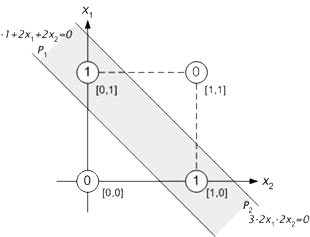
\includegraphics[height=7em]{figures/XOR.png}
				\end{figure}
			\end{columns}
		\end{itemize}
	\end{frame}

	\begin{frame}{Solution of XOR problem}
		\begin{itemize}
			\item Why linear model cannot deal with XOR problem?
			\item Solution? Nonlinear or \href{http://colah.github.io/posts/2014-03-NN-Manifolds-Topology/img/spiral.1-2.2-2-2-2-2-2.gif}{\underline{transform space}}!
			\begin{exampleblock}{Figures from \href{http://colah.github.io/posts/2014-03-NN-Manifolds-Topology/}{\underline{colah's blog}}}
				\begin{columns}[onlytextwidth]
					\column{0.33\textwidth}
					\begin{figure}
						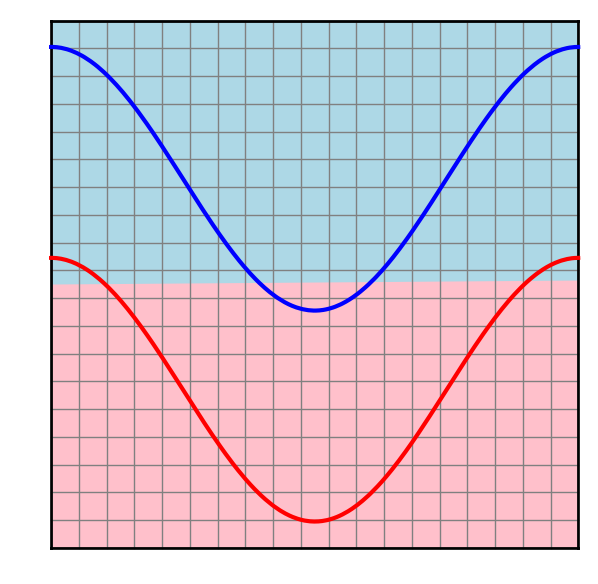
\includegraphics[height=8em]{figures/nonlinear-separable-1.png}
					\end{figure}
					
					\column{0.33\textwidth}
					\begin{figure}
						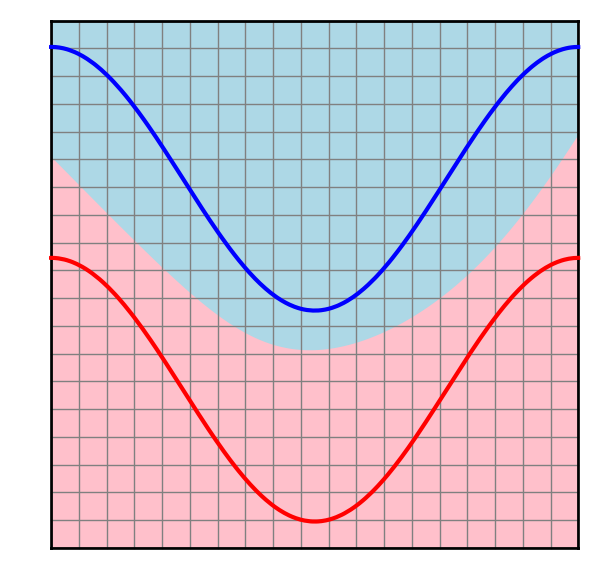
\includegraphics[height=8em]{figures/nonlinear-separable-2.png}
					\end{figure}
					
					\column{0.33\textwidth}
					\begin{figure}
						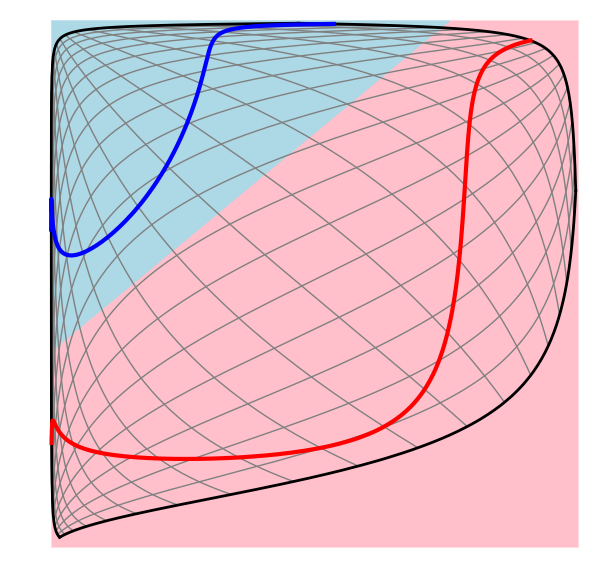
\includegraphics[height=8em]{figures/nonlinear-separable-3.png}
					\end{figure}
				\end{columns}
			\end{exampleblock}
			\item One way to solve this problem is to use a model that learns a different feature space in which a linear model is able to represent the solution.
			\item Non-linear models: Neural Networks, SVM, etc.
		\end{itemize}
	\end{frame}

	\begin{frame}{A simple feedforward network}
		\begin{columns}[T]
			\column{0.6\textwidth}
			\begin{itemize}
					\item A vector of hidden units $\bm{h}$ that are computed by a function $f^{\,(1)}(\bm{x};\bm{W},\bm{c})$
					\item The values of these hidden units are then used as the input for a second layer.
					\item The second layer is the output layer of the network.
					\item The output layer is still just a linear regression model, but now it is applied to $\bm{h}$ rather than to $\bm{x}$.
					\item The network now contains two functions chained together: $\bm{h}=f^{\,(1)}(\bm{x};\bm{W},\bm{c})$ and $y=f^{\,(2)}(\bm{h};\bm{w},b)$.
					\item the complete model is: $f(\bm{x};\bm{W},\bm{c},\bm{w},b)=f^{\,(2)}(f^{\,(1)}(\bm{x}))$
			\end{itemize}
		
			\column{0.4\textwidth}
			\begin{figure}
				\caption{A feedforward network with one hidden layer and two hidden units}
				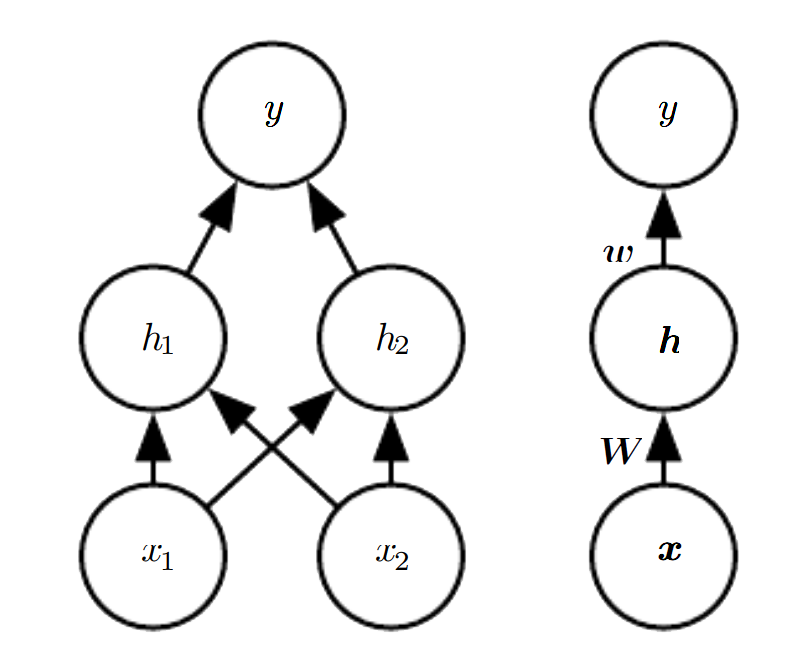
\includegraphics[height=10em]{figures/network-one-hidden-layer-two-hidden-unit.png}
			\end{figure}
		\end{columns}
	\end{frame}

	\begin{frame}{A simple feedforward network}
		\begin{columns}[T]
			\column{0.6\textwidth}
			\begin{itemize}
				\item $\bm{h}=f^{\,(1)}(\bm{x};\bm{W},\bm{c})$ and $y=f^{\,(2)}(\bm{h};\bm{w},b)$
				\item What function should $f^{\,(1)}$ compute? We may be tempting to make $f^{\,(1)}$be linear as well?
				\item Unfortunately, if $f^{\,(1)}$ were linear, then the feedforward network as a whole would remain a linear function of its input.
				\item suppose $f^{\,(1)}(\bm{x})=\bm{W}^T\bm{x}$ and $f^{\,(2)}(\bm{h})=\bm{h}^T\bm{w}$. Then $f(\bm{x})=\bm{w}^T\bm{W}^T\bm{x}$. We could represent this function as $f(\bm{x})=\bm{x}^T\bm{w'}$ where $\bm{w'}=\bm{Ww}$
				\item Clearly, we must use a nonlinear function to describe the features.
			\end{itemize}
			
			\column{0.4\textwidth}
			\setcounter{figure}{\thefigure-1}
			\begin{figure}
				\caption{A feedforward network with one hidden layer and two hidden units}
				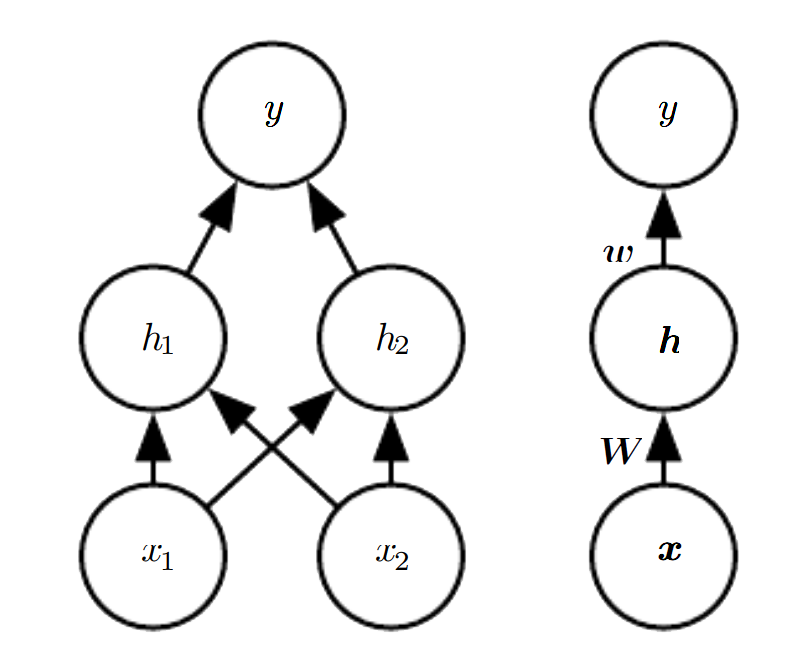
\includegraphics[height=10em]{figures/network-one-hidden-layer-two-hidden-unit.png}
			\end{figure}
		\end{columns}
	\end{frame}

	\begin{frame}{Activation Function}
		\begin{itemize}
			\item Most neural networks describe the features using an affine transformation controlled by learned parameters, followed by a fixed, nonlinear function called an \emph{activation function}.
			\item We define: $\bm{h}=g(\bm{W}^T\bm{x}+\bm{c})$, where $\bm{W}$ provides the weights of a linear transformation and $\bm{c}$ the biases.
			\item The activation function $g$ is typically chosen to be a function that is applied element-wise, with $h_i=g(\bm{x}^T\bm{W}^{:,i}+c_i)$.
			\item In modern neural networks, the default recommendation is to use the \emph{rectified linear unit} or ReLU (\citet{jarrett2009best,nair2010rectified,glorot2011deep}) defined by the activation function $g(z)=\max\{0,z\}$
			\begin{figure}
				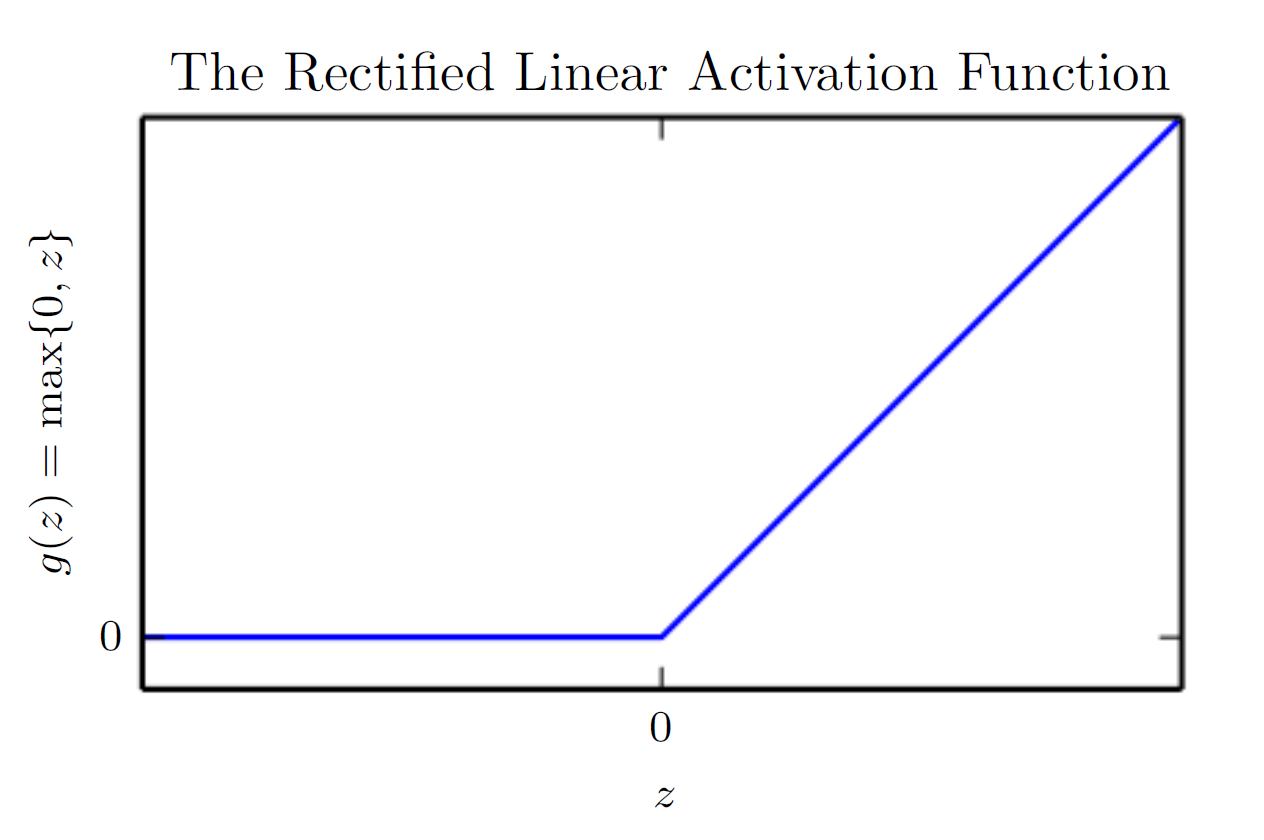
\includegraphics[height=7em]{figures/ReLU.png}
			\end{figure}
		\end{itemize}
	\end{frame}

	\begin{frame}{Solution of XOR problem}
		We can now specify our complete network as
		\begin{equation*}
			f(\bm{x};\bm{W},\bm{c},\bm{w},b)=\bm{w}^T\max\{0,\bm{W}^T\bm{x}+\bm{x}\}+b
		\end{equation*}
		We can now specify a solution to the XOR problem. Let
		\begin{eqnarray*}
			\bm{W}=\begin{bmatrix}
			1&1\\
			1&1
			\end{bmatrix}, 
			\bm{c}=\begin{bmatrix}
				0\\
				-1
			\end{bmatrix},
			\bm{w}=\begin{bmatrix}
				1\\
				-2
			\end{bmatrix}, b=0
		\end{eqnarray*}
		
		Let $\bm{X}$ be the design matrix containing all four points in the binary input space:
		$$\bm{x}=\begin{bmatrix}
		0&0\\
		0&1\\
		1&0\\
		1&1
		\end{bmatrix}$$
	\end{frame}

	\begin{frame}{Solution of XOR problem}
		The first step in the neural network is to multiply the input matrix by the first layer's weight matrix:
		
		$$\bm{XW}=\begin{bmatrix}
		0&0\\
		1&1\\
		1&1\\
		2&2
		\end{bmatrix}$$
		
		Next, we add the bias vector $\bm{c}$, to obtain:
		
		$$\bm{XW}+\bm{c}=\begin{bmatrix}
		0&-1\\
		1&0\\
		1&0\\
		2&1
		\end{bmatrix}$$
	\end{frame}

	\begin{frame}{Solution of XOR problem}
		To finish computing the value of $\bm{h}$ for each example, we apply the rectified linear transformation and then, we can use a linear model to solve the problem. We finish by multiplying by the weight vector $\bm{w}$
		$$\mathrm{ReLU}(\bm{XW}+\bm{c})=\begin{bmatrix}
		0&0\\
		1&0\\
		2&0\\
		2&1
		\end{bmatrix};\qquad\mathrm{ReLU}(\bm{XW}+\bm{c})\times \bm{w}=\begin{bmatrix}
		0\\
		1\\
		1\\
		0
		\end{bmatrix};$$
		
		The neural network has obtained the correct answer for every example in the batch.
		
		In this example, we simply specified the solution, then showed that it obtained zero error. In a real situation, there might be billions of model parameters and billions of training examples, so one cannot simply guess the solution as we did here.
		
		Instead, a \emph{gradient-based optimization algorithm} can find parameters that produce very little error.
	\end{frame}


	\begin{frame}[allowframebreaks]{References}
		\bibliography{Chap6}
		\bibliographystyle{plainnat}
	\end{frame}

\end{document}